\subsection{Auswahl des Experimentes und physikalischer Hintergrund}
\label{sec-2-3}
Welches Experiment unterstützt und welche physikalischen Zusammenhänge damit vermittelt werden sollen, bestimmt die inhaltlichen Aspekte einer Lösung. Helmholtz-Spulen werden sowohl in der Laborpraxis als auch in der schulischen und universitären Ausbildung verwendet. Beispielsweise wird mit ihnen in Schülerversuchen die Stärke des Erdmagnetfeldes bestimmt. Im Folgenden sollen die physikalischen Hintergründe kurz eingeführt sowie der Aufbau und Ablauf des Experimentes erläutert werden.\\

Zuvor soll jedoch kurz auf die Auswahl des vorgestellten Versuches eingegangen werden.

\subsubsection{Auswahl des Experimentes}
\label{sec-2-3-1}
Das Experiment wurde aus mehreren Gründen für diese Arbeit ausgewählt. Zum einen ist Augmented Reality für die Darstellung von Magnetfeldern eine gut geeignete Methode \cite{Buchau09}. Die im vorangegangen Abschnitt vorgestellten Arbeiten auf dem Gebiet motivieren den Einsatz der Technik in diesem Kontext. Aus dieser Perspektive ist das Experiment mit der Helmholtz-Spule geeignet, da die entstehenden Magnetfelder dabei im Fokus stehen. Außerdem bietet der Anwendungsfall Potential zur Erweiterung um andere Experimente mit einer Helmholtz-Spule. Aber auch weitere, teilweise komplexere Inhalte wie z.B. das Biot-Savart-Gesetz ließen sich daran anknüpfen.\\

Neben diesen Motivationen wurde der Versuch auch aus technischen und praktischen Aspekten ausgewählt. Im Wesentlichen trugen dazu die folgenden Faktoren bei:
\begin{itemize}
	\singlespacing
	\item Das Magnetfeld der Spule hat keine erkennbaren Auswirkungen auf die HoloLens (das Gerät nutzt ein Magnetometer). Bei im Vorfeld der Arbeit durchgeführten Versuchen mit Flussdichten von über 100 Mikrotesla konnten keine wahrnehmbaren Auswirkungen auf das Tracking und die Stabilität von Hologrammen festgestellt werden.
	\item Die notwendigen Materialien (Spule, Messgeräte, Simulationslösung) standen für diese Arbeit zur Verfügung.
	\item Die gegebene Größe der Spule (Radius von 15 cm) eignet sich für das beschränkte Sichtfeld der HoloLens.
	\item Das Experiment enthält keine sich schnell bewegenden Elemente und ist bis auf den Kompass statisch. Es erfordert außerdem keine Schutzausrüstung.
	\item Die physikalischen Hintergründe des Versuches sind nicht zu komplex für den Rahmen dieser Arbeit.
\end{itemize}

Einige dieser Umstände begünstigen einen Einsatz der Brille für diesen konkreten Anwendungsfall und sind ggf. bei anderen Szenarien so nicht gegeben.\\

\subsubsection{Spulen und Magnetfelder}
\label{sec-2-3-2}
Ein Magnetfeld kann als dreidimensionales Vektorfeld aufgefasst werden. Die Stärke an einem Punkt lässt sich über den Feldstärkevektor $\boldsymbol{H}$ sowie die Flussdichte $\boldsymbol{B}$ angeben. Beide Größen hängen über eine die magnetische Feldkonstante $\mu_{0}$ zusammen: $\boldsymbol{B} = \mu_{0} \cdot \boldsymbol{H}$.
\par
\noindent\hspace*{5mm}
Wird eine Leiterschleife von einem elektrischen Strom durchflossen, so induziert diese ein Magnetfeld. Dieses Feld verläuft sowohl durch das Innere als auch durch die Umgebung der Spule. Die Stärke des Feldes hängt dabei von der Windungszahl und dem Durchmesser der Spule sowie der anliegenden Stromstärke ab.
Im Zentrum der Spule ist das Magnetfeld \textit{homogen}. Das bedeutet, es ist an allen Punkten im Raum gleich stark und gleich gerichtet. Außerhalb und am Rand der Spule hingegen ist das Feld \textit{inhomogen}, es erfüllt beide zuvor genannten Eigenschaften nicht.\\

\textbf{Darstellungsformen von Magnetfeldern}\\
Zur Visualisierung von Magnetfeldern gibt es unterschiedliche Darstellungsmodelle. Im Bereich der Lehre haben sich davon vor allem zwei etabliert: Feldlinien und Vektoren. Beide stellen das Feld mit Richtung und Stärke im Raum dar, unterscheiden sich aber in der Art und Weise.\\ %Abbildung \ref{img:Magnetfeld-Helmholtzspule} zeigt eine gemeinsame Darstellung beider Ansätze für eine Helmholtz-Spule.\\

\begin{comment}
\begin{figure}[h!]
	\centering
	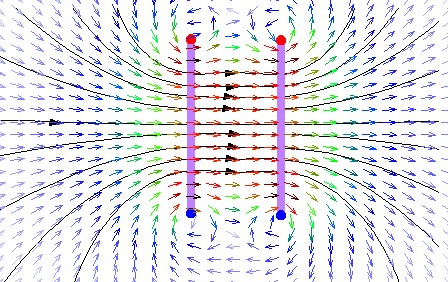
\includegraphics[width=0.65\textwidth]{images/papers/Magnetfeld-Helmholtzspule.jpg}
	\caption{Magnetfeld einer Helmholtz-Spule in der X-Z-Ebene \cite{wiki:15}. Statt über die Vektorlänge wurde der Betrag des Feldes hier mittels Farben visualisiert. Die Feldlinien sind für einen mittigen Ausschnitt der Spule gezeichnet. Im Inneren ist das Feld weitgehend homogen.} %\footnote{\url{https://de.wikipedia.org/wiki/Helmholtz-Spule}}}
	\label{img:Magnetfeld-Helmholtzspule}
\end{figure}
\end{comment}

\textit{Das Feldlinienmodell}\\
Die Feldliniendarstellung ist weit verbreitet und wurde in allen zuvor vorgestellten AR-Lösungen verwendet. Das Modell bildet den magnetischen Fluss auf kontinuierliche Linien ab. Die Tangente an einem Punkt der Feldlinie entspricht der Richtung des Feldstärkevektors diesem Punkt. Die Stärke des Feldes wird meist proportional zur Dichte der Feldlinien dargestellt \cite{Kilian03}.\\

Diese Darstellung macht den Unterschied zwischen homogenen und inhomogenen Feldern besonders gut sichtbar, da bei einem homogenen Feld die Feldlinien parallel verlaufen, bei einem inhomogenen hingegen nicht. Außerdem ist die Darstellung über die Dichte der Feldlinien eng verbunden mit dem Konzept des magnetischen Flusses.\\

Allerdings bedeutet diese Darstellungsform auch, dass mit zunehmender Feldstärke zunehmend mehr Feldlinien auf gleichem Raum dargestellt werden müssen. Außerdem ist bei sich ändernden Feldern schwer zu erkennen, ob sich nur die Beträge der Feldstärkevektoren ändern, oder auch deren Richtungen. Denn in beiden Fällen verändern sich Form und Abstand der Feldlinien.\\

\textit{Vektorfeld}\\
In der Vektor-Darstellung wird das Feld über einzelne Vektoren repräsentiert. Dabei geben Richtung und Betrag eines Vektors den Feldstärkevektor des Magnetfeldes für einen Punkt im Raum an.\\
So lässt sich die Feldstärke an einem durch einen Vektor repräsentierten Punkt im Raum direkt ablesen. Wo ein Feld homogen ist lässt sich jedoch nur durch das Vergleichen von mehreren Vektoren in Länge und Richtung feststellen. Dieses Modell hat gegenüber dem Feldlinienmodell jedoch den Vorteil, dass mit zunehmender Feldstärke die Vektoren nur länger werden, ihre Anzahl jedoch gleich bleibt. Außerdem ist hier klar zu erkennen, ob bei einem sich ändernden Feld die Richtung der Vektoren konstant bleibt, oder nicht.

\subsubsection{Helmholtz-Spule}
\label{sec-2-3-3}
Bei einer Helmholtz-Spule handelt es sich im Prinzip um zum zwei zusammengeschaltete Spulen. Dabei werden zwei identische Spulen parallel nebeneinander aufgestellt, sodass der Abstand genau dem Radius der Spulen entspricht. Abbildung \ref{img:Helmholtz} zeigt eine solche Helmholtz-Spule.\\
\begin{wrapfigure}{r}{0.4\textwidth}
	\centering
	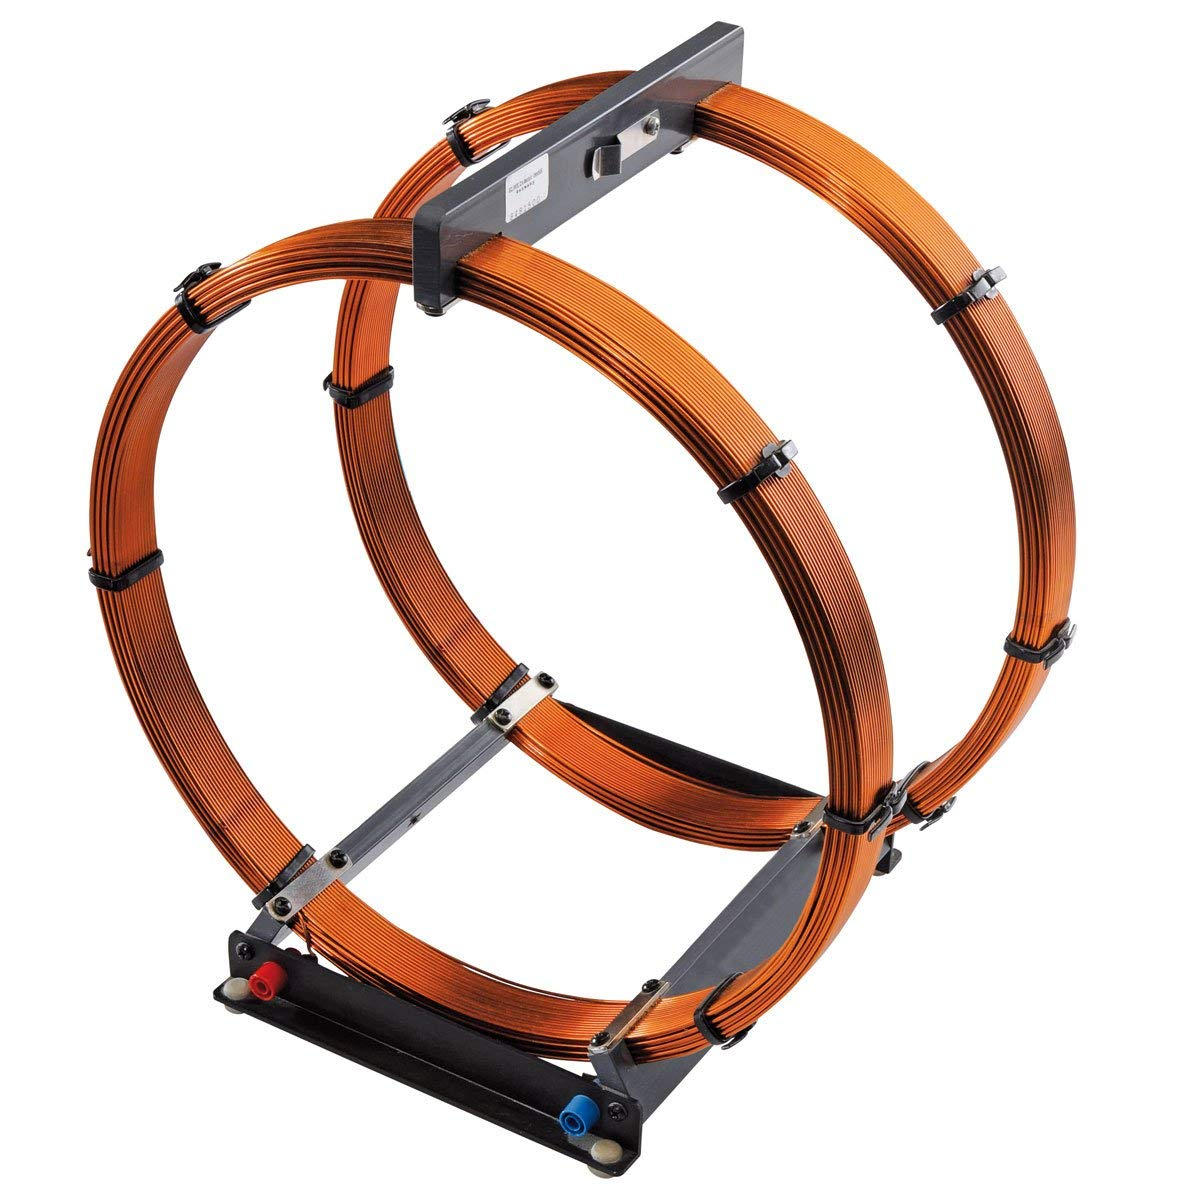
\includegraphics[width=0.38\textwidth]{images/papers/Helmholtz.jpg}
	\caption{Foto der verwendeten Helmholtz-Spule. Radius und Abstand betragen 15 cm und jede Teilspule hat 124 Windungen \cite{3BS}.}
	\label{img:Helmholtz}
\end{wrapfigure}

Durch diese spezielle Eigenschaft des Aufbaus überlagern sich die beiden, durch die einzelnen Spulen entstehenden Magnetfelder genau so, dass im Raum zwischen den Spulen ebenfalls ein (nahezu) homogenes Magnetfeld entsteht. Lediglich am Rand und in unmittelbarer Nähe zu den Spulen wird das Feld zunehmend inhomogen. Die Zeichnung in Abbildung \ref{img:hh-mfeld} zeigt diesen Zusammenhang für die Spulenachse. Detailliertere Informationen dazu finden sich beispielsweise in \cite{Demtroder13}.\\

\begin{wrapfigure}{r}{0.5\textwidth}
	\centering
	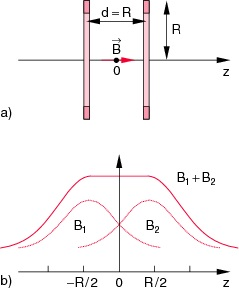
\includegraphics[width=0.48\textwidth]{images/papers/BiotSavart.jpg}
	\caption{Oben: Skizze des Spulenpaars. Unten: Betrag der Flussdichte des entstehenden Feldes entlang der Z-Achse. Zwischen den Spulen ist das Feld nahezu homogen \cite{Demtroder13}.}
	\label{img:hh-mfeld}
\end{wrapfigure}


Das Feld wird durch elliptische Integrale beschrieben, die nur numerisch zu lösen sind. Im Mittelpunkt zwischen den Spulen vereinfacht sich die Feldgleichung jedoch zu folgender Gleichung:
\begin{equation}
\label{eq:mfield}
B = \mu_{0} \cdot \frac{8 \cdot I \cdot N}{\sqrt{125} \cdot R}
\end{equation}

Dabei entspricht $I$ der Stromstärke, $N$ der Windungszahl, $R$ dem Radius und $\mu_{0}$ der magnetischen Feldkonstanten. Die Stromstärke tritt in der Feldgleichung nur als linearer Faktor auf. Änderungen an der Stromstärke rufen also eine dazu proportionale Änderung der Flussdichte hervor. Außerdem bedeutet dieser Umstand, dass die Richtung des Feldstärkevektors nicht von der Stromstärke abhängt, sondern konstant bleibt.\\

\subsubsection{Versuchsaufbau und Versuchsablauf}
\label{sec-2-3-4}
Ziel des Versuches ist die Bestimmung des Erdmagnetfeldes. Genauer bedeutet das die experimentelle Bestimmung von Richtung und Stärke des magnetischen Flussdichtevektors. Die Richtung kann dabei allein über den Kompass bestimmt werden. Der Betrag der Flussdichte wird mittels Gleichung \ref{eq:mfield} aus der gemessenen Stromstärke ermittelt, bei der die Helmholtz-Spule ein gleich starkes, eigenes Magnetfeld erzeugt.\\

\textit{Aufbau}\\
Der Versuchsaufbau ist in Abbildung \ref{img:experiment-devices} dargestellt und besteht aus: 
\begin{itemize}
	\setlength{\itemsep}{-5pt}
	\item Einer Helmholtz-Spule mit fester Windungszahl und festem Radius
	\item Einem mittig in der Spule positionierten Kompass
	\item Einem in Reihe geschalteten Amperemeter
	\item Einem in Reihe geschalteten Widerstand	
	\item Einer angeschlossenen Spannungsquelle
\end{itemize}

\begin{figure}[h!]
	\centering
	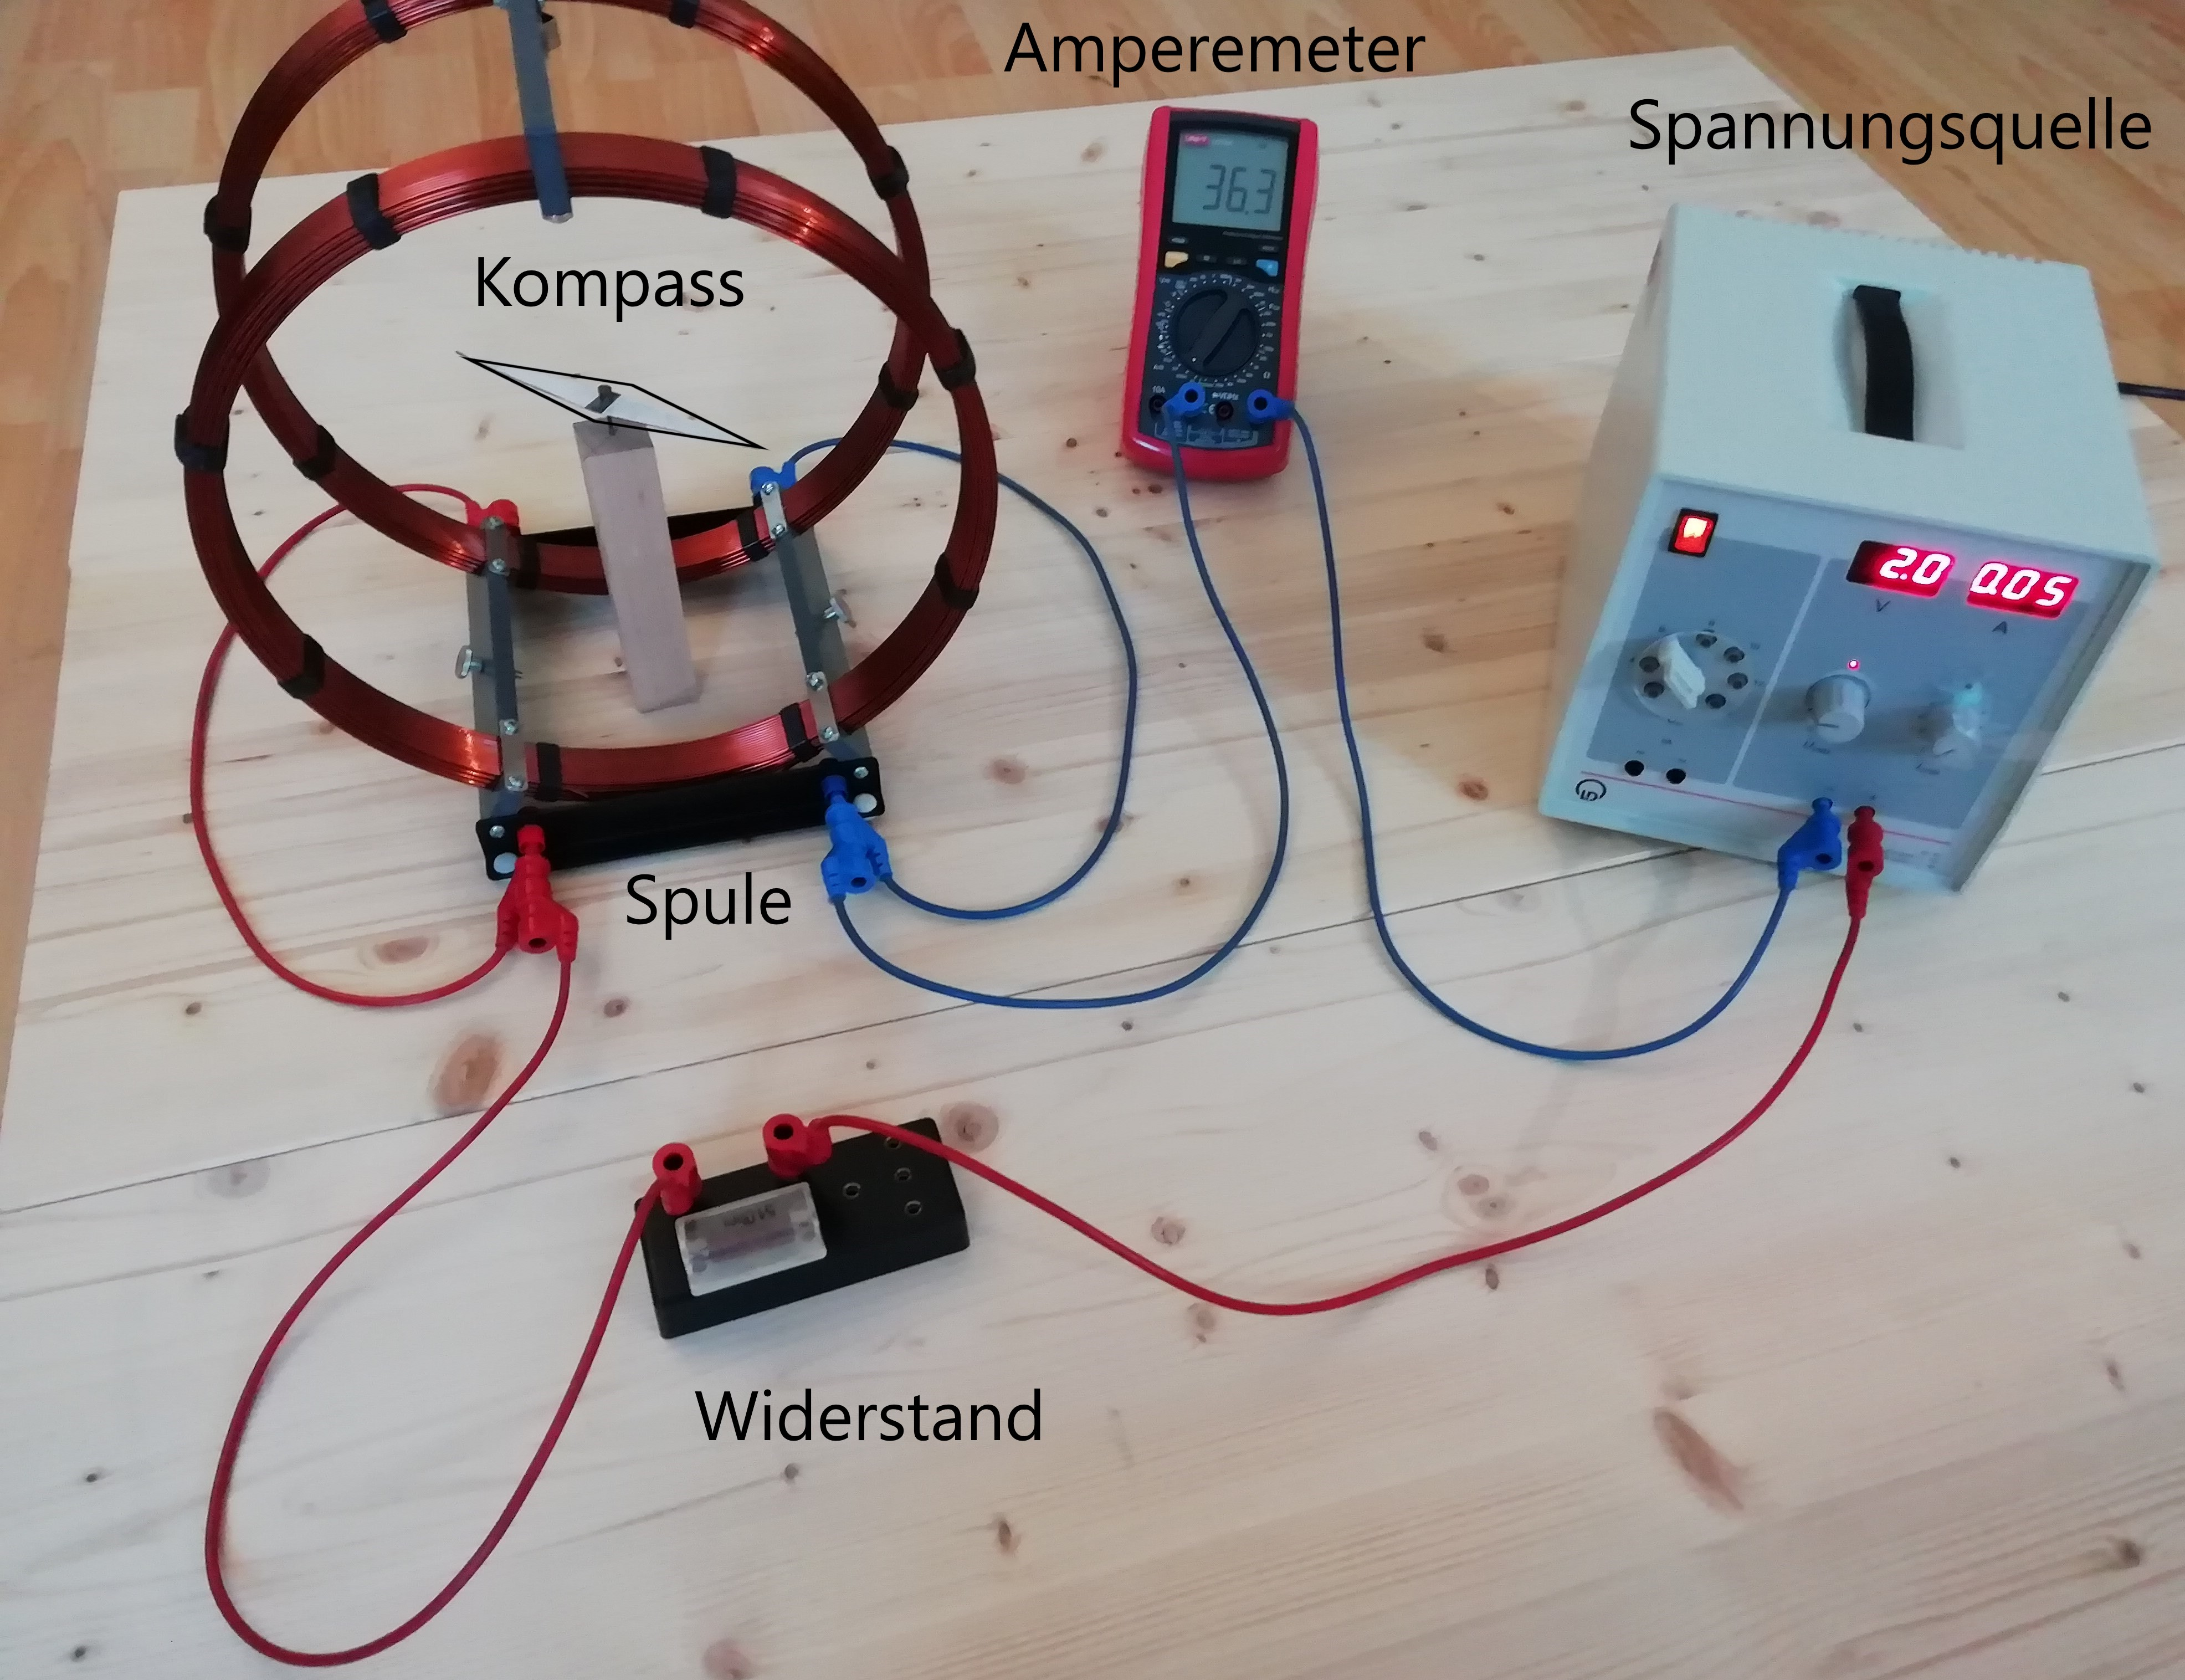
\includegraphics[width=0.8\textwidth]{images/papers/setup_labled.jpg}
	\caption{Foto des Versuchsaufbaus. Die Helmholtz-Spule besteht aus zwei parallel geschalteten Spulen. Der Widerstand passt den Bereich der einstellbaren Stromstärke an. Der weiß überklebte Kompass wurde nachträglich schwarz umrandet, damit er auf dem Foto besser zu sehen ist.}
	\label{img:experiment-devices}
\end{figure}

\textit{Ablauf}\\
Der Versuch läuft in zwei Teilen ab. Zunächst wird die Ausrichtung des Erdmagnetfeldes bestimmt und im nächsten Schritt dann der Betrag der Flussdichte. Der Ablauf lässt sich wie folgt zusammenfassen:
\begin{enumerate}
	\setlength{\itemsep}{-2pt}
	\item Kompassnadel nach Norden ausrichten lassen
	\item Helmholtz-Spule orthogonal zur Kompassnadel ausrichten
	\item Spannungsquelle einschalten und Spannung langsam erhöhen
	\item Spannung erhöhen, bis Kompassnadel um 45° ausgelenkt ist
	\item Stromstärke ablesen und in Gleichung \eqref{eq:mfield} einsetzen
\end{enumerate}

Durch dieses Vorgehen wird im zweiten Schritt durch die Spule ein Magnetfeld erzeugt, das orthogonal zu dem der Erde gerichtet ist. Beide Felder überlagern sich, so dass sie den Kompass genau dann gleichmäßig in beide Richtungen auslenken, wenn beide Felder gleich stark auf die Nadel wirken.

